% -*- compile-command: "cd .. && make" -*-
\documentclass[document.tex]{subfiles}
\begin{document}

\chapter{Platform Manuals}
\label {ch:appendix-manuals}


\sectionnote {BM}
\section{Expirable}
\label {sec:expirable-manual}

Expirable is a simple Rails mixin to handle deadlines in workflows.
It builds on \href{https://github.com/collectiveidea/delayed\_job}{Delayed::Job}
and \href{https://github.com/tomykaira/clockwork}{Clockwork} to provide a painless approach
to handling time-based events.

\subsection{Installation}

To install the Expirable and its dependencies, add {\tt expirable} and an
appropriate Delayed::Jobs backend to your Gemfile:

\begin{lstlisting}
gem 'delayed_job_active_record'
gem 'expirable'

\end{lstlisting}   %  class="language-ruby"

Next, set up Delayed::Job if you are not already using it in your project:

\begin{lstlisting}
rails generate delayed_job:active_record
rake db:migrate

\end{lstlisting}   %  class="language-bash"

Finally, set up Expirable itself by running {\tt rails g expirable:setup}.
This will create a Clockwork configuration file called \emph{lib/clock.rb}.
By default, it is configured to check deadlines at one minute past every hour.
See the \href{https://github.com/tomykaira/clockwork\#clockwork---a-clock-process-to-replace-cron--}{Clockwork manual}
for more information if you need to change this configuration.

\subsection{Running Expirable}

To run Expirable, you will need to run a Clockwork worker and a Delayed::Job worker.
You can run the Clockwork worker by executing {\tt bundle exec clockwork lib/clock.rb}
from the root of the Rails project, and Delayed::Job worker with {\tt ./bin/delayed\_job run}.

You can also use \href{http://blog.daviddollar.org/2011/05/06/introducing-foreman.html}{Foreman}
to manage these processes. For example, if you run your Rails application on Unicorn, then
you can create a {\tt Procfile} with the following content and run your application with {\tt foreman start}:

\begin{lstlisting}
cron: bundle exec clockwork lib/clock.rb
web: bundle exec unicorn_rails
worker: ./bin/delayed_job run

\end{lstlisting}   %  class="language-conf"

\subsection{Handling Deadlines}

To be expirable, a class must do the following three things:

\begin{enumerate}
\item include {\tt Expirable};
\item define a {\tt deadline\_expired} instance method that will be invoked when the model's deadline expires; and
\item define a class method named {\tt newly\_expired} that returns a collection of model instances that have expired, but haven't yet received a {\tt deadline\_expired} message.
\end{enumerate}

\pagebreak

As an example, the following model uses \href{https://github.com/aasm/aasm}{AASM} and Expirable to transition tasks to a failed state when their deadline is passed:

\begin{lstlisting}
class ExampleTask < ActiveRecord::Base
  include AASM
  include Expirable
  
  scope :newly_expired,
        -> { in_progress.where('deadline < ?', DateTime.now) }

  aasm do
    # ... state and event definitions skipped ...

    event :deadline_expired do
      transitions from: :in_progress, to: :missed
    end
  end
end

\end{lstlisting}   %  class="language-ruby"


\sectionnote {BM}
\section{aasm\_statecharts}
\label{sec:aasm-statecharts-manual}

{\tt aasm\_statecharts} is a utility for generating UML statechart diagrams from state machines defined using \href{https://github.com/aasm/aasm}{AASM}. Unlike other state diagram generators, it can express extended finite state machine concepts such as guards and entry actions.

\subsection{Installation and Invokation}

You can install {\tt aasm\_statecharts} from RubyGems using {\tt gem install aasm\_statecharts}, or add the {\tt aasm\_statecharts} gem to your Gemfile and run Bundler to install it.

If you have installed {\tt aasm\_statecharts} via gem, you can invoke it using the command {\tt aasm\_statecharts}; otherwise, if you have used Bundler without generating binstubs, you can invoke it with the command {\tt bundle exec aasm\_statecharts}. The following assumes that it has been installed via gem for simplicity.

\pagebreak

\subsection{Example}

Considuer following model, which is assumed to be stored in {\tt app/models/claim.rb}:
\begin{lstlisting}
class Claim < ActiveRecord::Base
  belongs_to :user
  validates :title, presence: true
  validates :description, presence: true

  include AASM
  aasm do
    state :unsubmitted, initial: true
    state :submitted, exit: [:cancel_deadline, :close_ticket]
    state :resolved, final: true

    event :submit do
      transitions from: :unsubmitted, to: :submitted,
                  guard: :accepting_claims?,
                  on_transition: :notify_submitted
    end
    event :return do
      transitions from: :submitted, to: :unsubmitted
    end
    event :accept do
      transitions from: :submitted, to: :resolved
    end
  end

  def accepting_claims?
  end
  def cancel_deadline
  end
  def close_ticket
  end
  def notify_submitted
  end
end
\end{lstlisting}

\pagebreak

If we invoke {\tt aasm\_statecharts claim}, then the following diagram will be written to ./doc/claim.png:

\vspace{5mm}

\begin{center}
 \includegraphics[width=3.0in]{./img/manual/aasm-statecharts-claim}
\end{center}


\subsection{Usage}

For more advanced usage information, see {\tt aasm\_statecharts --help}:

\begin{verbatim}Usage: aasm_statecharts [options] <model> [models ...]
    -a, --all                        Render all models using AASM
    -d, --directory directory        Output to a specific directory
     (default: ./doc)
    -t, --file-type type             Output in the specified format
     (default: png), which must be one of the following: bmp, canon,
     dot, xdot, cmap, dia, eps, fig, gd, gd2, gif, gtk, hpgl, ico,
     imap, cmapx, imap_np, cmapx_np, ismap, jpeg, jpg, jpe, mif, mp,
     pcl, pdf, pic, plain, plain-ext, png, ps, ps2, svg, svgz, tga,
     tiff, tif, vml, vmlz, vrml, vtx, wbmp, xlib, none.
\end{verbatim}



\sectionnote {BM}
\section{aasm\_progressable}
\label {sec:aasm-progressable-manual}

{\tt aasm\_progressable} is a Rails helper to render the progress indicators for simple linear \href{https://github.com/aasm/aasm}{AASM} workflows. It also provides predicates to make it easy to check a model's current position in its workflow. Using {\tt aasm\_progressable} allows users to see steps in a workflow they have completed, which step is in progress, and which steps have not been completed. See the following image for an example.

\vspace{5mm}

\begin{center}
 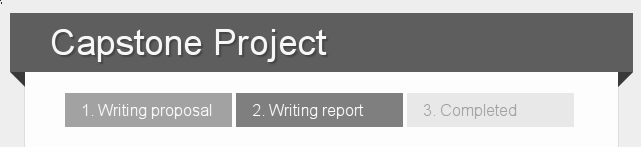
\includegraphics[width=6.0in]{./img/manual/aasm-progressable-example}
\end{center}

\subsection{Usage}

Add {\tt aasm\_progressable} to your Gemfile, and run bundler to install it. For each model with an appropriate workflow, include {\tt AasmProgressable::ModelMixin}, and add a call to {\tt aasm\_state\_order} with an array of symbols corresponding to
the expected order in which the states will be traversed. For example, if you have an {\tt Order} class that starts from the {\tt new} state, proceeds to {\tt processing}, and then {\tt shipping}, you might have

\pagebreak

\begin{lstlisting}
class Order < ActiveRecord::Base
  include AASM
  aasm do
    state :new, initial: true
    state :processing
    state :shipping
    
    event :confirm do
      transitions from: :new, to: :processing
    end
    event :dispatch do
      transitions from: :processing, to: :shipping
    end
  end
  
  aasm_state_order [:new, :processing, :shipping]
end

\end{lstlisting}   %  class="language-ruby"

In order to render the progress indicator, you need to add \\ {\tt helper AasmProgressable::Helper} to your ApplicationController. Then in any detailed views for the order (such as {\tt orders\#show}), add {\tt \textless{}\%= render\_state\_indicator the\_model\_instance \%\textgreater{}} to render an indicator for the state of the specified instance of the model. By default, this will render an ordered list ({\tt ol}) with one element per state, with the elements corresponding to complete, current, and incomplete states being classed with {\tt complete}, {\tt active}, and {\tt incomplete} respectively. You can add a ` *= require aasm\_progressable` line to your application stylesheet to include some default styling for the indicator.

\subsection{Custom Rendering}

The default template for {\tt aasm\_progressable} can be customized to suit your needs. Run {\tt rails g aasm\_progressable:views} to copy the default template to \\ app/views/aasm\_progressable/states/\_list.html.erb, and then edit it as necessary.

If you need additional template variables, you can pass local variables to the invocation of {\tt render\_state\_indicator}. For instance, you can do the following to make the model instance available in a local variable:

\begin{lstlisting}
<%= render_state_indicator the_model_instance,
                           locals: {object: the_model_instance} %>

\end{lstlisting}   %  class="language-erb"

\subsection{Localization}

{\tt aasm\_progressable }uses {\tt AASM::Localizer\#human\_state\_name} to convert AASM states to output text. By default, this method will replace underscores with spaces, and capitalize the first letter of the state name. However, it can also fetch state names from a locale key of the form \\ {\small \tt activerecord.attributes.\textless{}model-table-name\textgreater{}.\textless{}aasm-column-name\textgreater{}/\textless{}state-symbol\textgreater{}}. By default, {\tt \textless{}aasm-column-name\textgreater{}} will be ``aasm\_state''.

As an example, if we wanted to display ``Unconfirmed'' as English name for the {\tt :new} order state in the previous example, we could add the following to config/locales/en.yml:

\begin{lstlisting}
en:
  activerecord:
    attributes:
      order:
        aasm_state/new: "Unconfirmed"

\end{lstlisting}   %  class="language-yaml"

\subsection{State Predicates}

{\tt aasm\_progressable} also provides a few predicates that you can use to query a model's state:

\begin{itemize}
\item {\tt \#have\_completed?} and {\tt \#have\_not\_completed?} can be used to check if a step has already been finished. In the Order example, if the current state of an instance named {\tt order} was {\tt processing}, then {\tt order.have\_completed? :new} would return true, while {\tt order.have\_completed? :processing} would return false.
\item {\tt \#have\_started?} and {\tt \#have\_not\_started?} can be used to check if a step has already started. Again using the Order model defined previously, if an instance named {\tt order} was in the {\tt processing} state, then {\tt order.have\_started? :processing} would be true, while {\tt order.have\_not\_started? :shipping} would return false.
\end{itemize}

\subsection{Limitations}

Models that use {\tt aasm\_progressable} should have a strictly linear workflow, ie. there should be no branches in the state machine. Loops and skipped states are permitted, but there may not be alternative states. If a model instance is in a state that does not appear in the model's {\tt aasm\_state\_order} declaration, then the helper will not be able to infer the state transition history of the instance and all states will be rendered as if they were completed.


\sectionnote {BM}
\section{aasm\_actionable}
\label {sec:aasm-actionable-manual}

aasm\_actionable is a Rails extension that helps factor out boilerplate state and authorization conditionals from view code. Using \href{https://github.com/elabs/pundit}{pundit} for authorization, it allows developers to write partials for user actions that are automatically displayed to the user if the model is in an appropriate state, and the user has sufficient permissions.

\subsection{Installation}

Add {\tt aasm\_actionable} to your Gemfile, and run Bundler to install it. You will also want to install Pundit, as described in the \href{https://github.com/elabs/pundit\#installation}{Pundit documentation}.

\subsection{Using aasm\_actionable}

Each action that aasm\_actionable may display requires the developer to provide three things:

\begin{enumerate}
\item An event with the same name as the desired action, ex. {\tt do\_action};
\item A method on the pundit policy for the model on which the action is to be performed, ex. {\tt do\_action?}; and
\item A partial view for the model with the same name as the action, ex. \\ {\tt mymodel/\_do\_action.html.erb}.
\end{enumerate}

Additionally, you may wish to create a controller method and route to handle the action being performed. By convention, the controller method should have the same name as the action, ie. {\tt do\_action} for the example above.

Once you have provided one or more actions for a model, you can render a model instance's available actions by including {\tt AasmActionable::ControllerMixin} in your controller, and adding {\tt \textless{}\%= render\_state\_actions my\_instance \%\textgreater{}} in your view. The default template uses styles and code from \href{http://getbootstrap.com/}{Bootstrap 3}, so you should either ensure that it is included in your application, or change the default template (see Custom Rendering below.) 

\subsection{Example}

Consider the following contrived Order model (in {\tt app/models/order.rb}) for a (trivial) online store:

\begin{lstlisting}
class Order < ActiveRecord::Base
  include AASM
  aasm do
    state :new, initial: true
    state :processing
    state :shipping

    event :confirm do
      transitions from: :new, to: :processing
    end
    event :dispatch do
      transitions from: :processing, to: :shipping
    end
  end
end

\end{lstlisting}   %  class="language-ruby"

Suppose that users in an inventory tracking role manually confirm an order by double-checking if the item is in stock, while users in shipping are responsible for marking an order as dispatched. We would like to render appropriate actions on a view of the order, depending on the order's state and the role that the user occupies. Confirmation does not add any new information to the order, but dispatching the order requires a shipping number.

First, we need to define an policy to describe which users can perform which actions. In {\tt app/policies/order.rb}, we create a new {\tt OrderPolicy} class, and define appropriate {\tt confirm?} and {\tt dispatch?} methods:

\begin{lstlisting}
class OrderPolicy < ApplicationPolicy
  # ... other default policy methods (ex. show?) omitted for brevity.

  def confirm?
    user.in_role? :inventory
  end

  def dispatch?
    user.in_role? :shipping
  end
end

\end{lstlisting}   %  class="language-ruby"

Next, we add methods to the order controller to handle these actions, along with the mixin:

\begin{lstlisting}
class OrderController < ApplicationController
  include AasmActionable::ControllerMixin

  # ... other controller methods omitted ...
  
  def show
    @order = find_order
    authorize @order
  end



  def confirm
    @order = find_order
    authorize @order

    if order.confirm!
      redirect_to order
    else
      # ... handle the error and re-render the order page ...
    end
  end
  
  def dispatch
    @order = find_order
    authorize @order
    
    dispatch_params = params.require(:order).permit(:shipping_number)
    order.assign_attributes(dispatch_params)

    if order.dispatch!
      redirect_to order
    else
      # ... handle the error and re-render the order page ...
    end
  end
  
  private
  
  def find_order
    Order.find(params[:id])
  end
end

\end{lstlisting}   %  class="language-ruby"

(You may want to consider using \href{https://github.com/plataformatec/responders}{responders} or a similar library to cut down on boilerplate in your custom controller methods.)

\pagebreak

We must also add the new actions to {\tt config/routes.rb}:

\begin{lstlisting}
  # ... other routes omitted ...
  
  resources :orders do
    member do
      post 'confirm'
      post 'dispatch'
    end
  end
  
  # ...

\end{lstlisting}   %  class="language-ruby"

Next, we create a partial for each action. For example, for the dispatch action we might write the following {\tt app/views/order/\_dispatch.html.erb}:

\begin{lstlisting}
<% form_for @order, url: dispatch_order_path, method: :post do %>
  <div>
    <%= f.label :shipping_number %>:
    <%= f.text_field :shipping_number %>
  </div>
  <%= f.submit "Dispatch" %>
<% end %>

\end{lstlisting}   %  class="language-erb"

Finally, we render the actions in the order view by adding {\tt \textless{}\%= render\_state\_actions @order \%\textgreater{}} to {\tt app/views/order/show.html.erb}.

\subsection{Custom Rendering}

The default template for {\tt aasm\_actionable} can be customized as necessary. Run {\tt rails g aasm\_actionable:views} to copy the template to \\ app/views/aasm\_actionable/\_list.html.erb, and edit it as required.

\end{document}